\documentclass[11pt, titlepage]{article}

\usepackage[margin=1in]{geometry}
\usepackage[strict]{changepage}
\usepackage{float}
\usepackage{fancyhdr}
\usepackage{mhchem}
\usepackage{siunitx}
\usepackage{wrapfig, booktabs}
\usepackage{enumitem}
\usepackage{caption}
\usepackage{commath}
\usepackage{amsmath}
\usepackage[hang]{footmisc}
\usepackage{multicol}
\usepackage{amsfonts}
\usepackage{mathrsfs}
\usepackage{mathtools}
\usepackage{tikz}

% my imports
\usepackage[most]{tcolorbox}
\usepackage{hyperref}
\hypersetup{
    colorlinks,
    citecolor=black,
    filecolor=black,
    linkcolor=black,
    urlcolor=black
}

\newcommand{\experimentDate}{\today}
\newcommand{\className}{CSE 371}
\newcommand{\assignmentname}{Lab 4}
\author{Cameron Jennings (ID: 2029631), Donovan Clay (ID: 2276005)}
\newcommand{\authorLastName}{Jennings, Clay}
\title{\assignmentname}

\date{\parbox{\linewidth}{\centering
\experimentDate
  \endgraf\bigskip
  \className\
}}

\pagestyle{fancy}
\fancyhf{}
\setlength{\headheight}{13.59999pt}
\rhead{\authorLastName\ \thepage}
% \lhead{\experimentShortName}
\lhead{\hyperref[beginning]{\assignmentname}}
\cfoot{\className\ -- \assignmentname}

\usepackage{color}
\usepackage{sectsty}

\definecolor{WordSectionBlue}{RGB}{30, 90, 147}

\allsectionsfont{\color{WordSectionBlue}}

\tcbuselibrary{breakable}


\begin{document}
	\maketitle
 
    \setcounter{tocdepth}{2}
    \begin{center}
        \tableofcontents\label{beginning}
    \end{center}
    \newpage
    
    \section{Design Procedure}
        In this lab, we gained practice implementing the control and datapath of a system for the purpose of programming algorithms in hardware. With this approach, the FSM for routing logic and the data storage/manipulation are separated to ensure that implementations are simplistic and scalable. We created two different systems following an algorithmic state machine and datapath design style, a bit-counter algorithm and a binary search algorithm.
    
        \subsection{Task \#1}
            The first task of the lab was to implement a system that counts the number of one bits in an 8 bit binary number. The DE1\_SoC board's switches are set to represent the 8 bit number using SW[7:0] (also known as the A input in the program) and the keys are used for the start and reset of the system using KEY[3] and KEY[0] respectively. The task also uses HEX0 and LEDR[9] to display the state of the system.

            \begin{figure}[H]
                \centering
                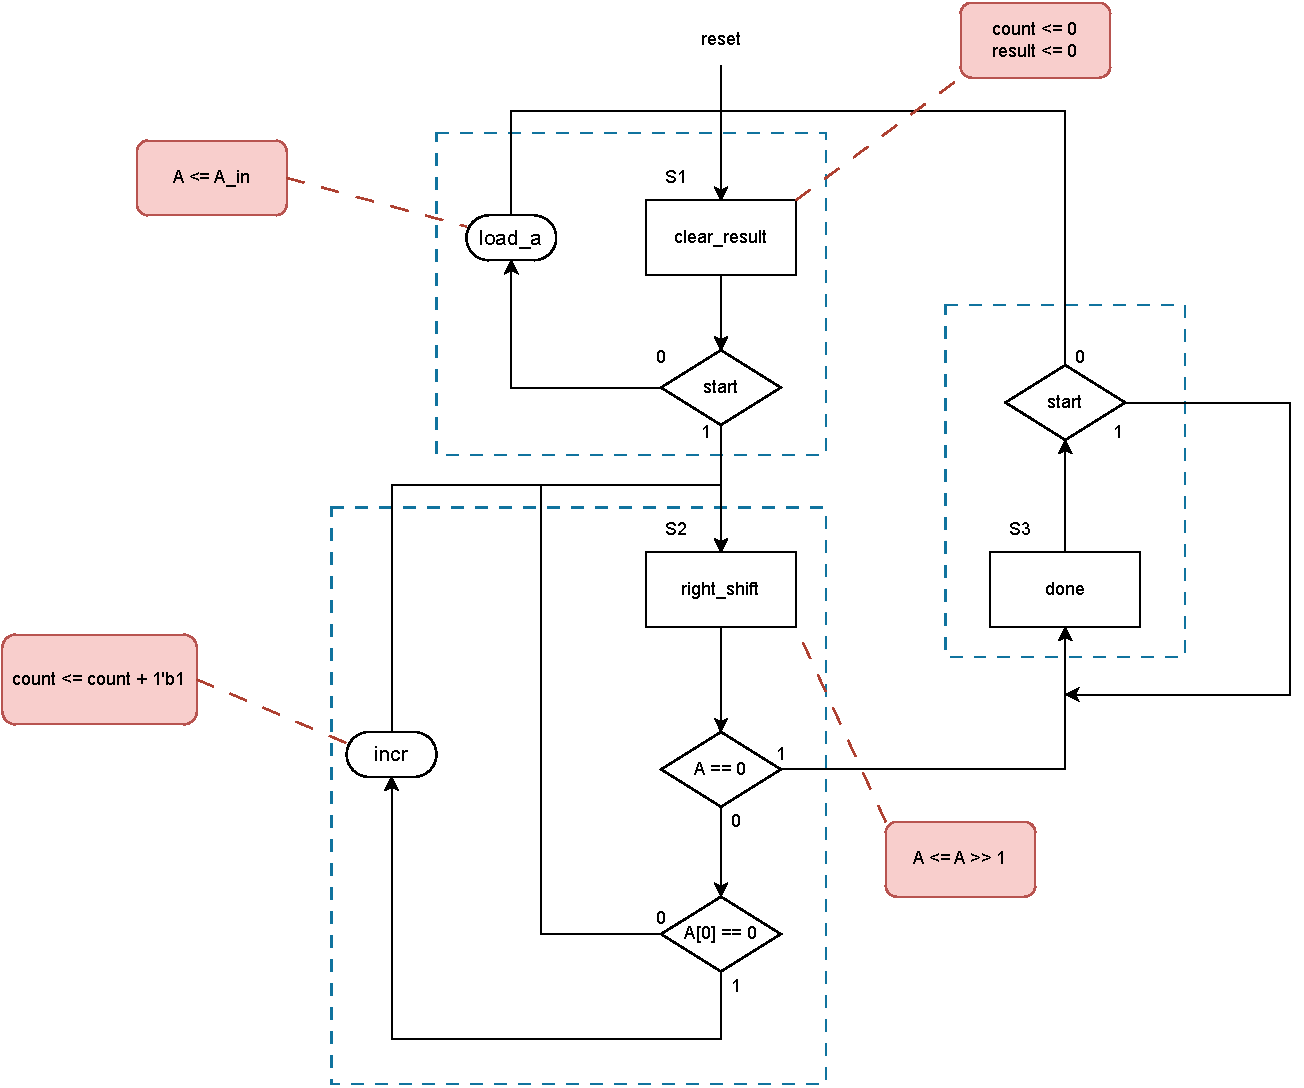
\includegraphics[scale = 0.7]{Images/task 1 asmd diagram.pdf}
                \caption{Bit-counter ASMD chart}
            \end{figure}

            \begin{figure}[H]
                \centering
                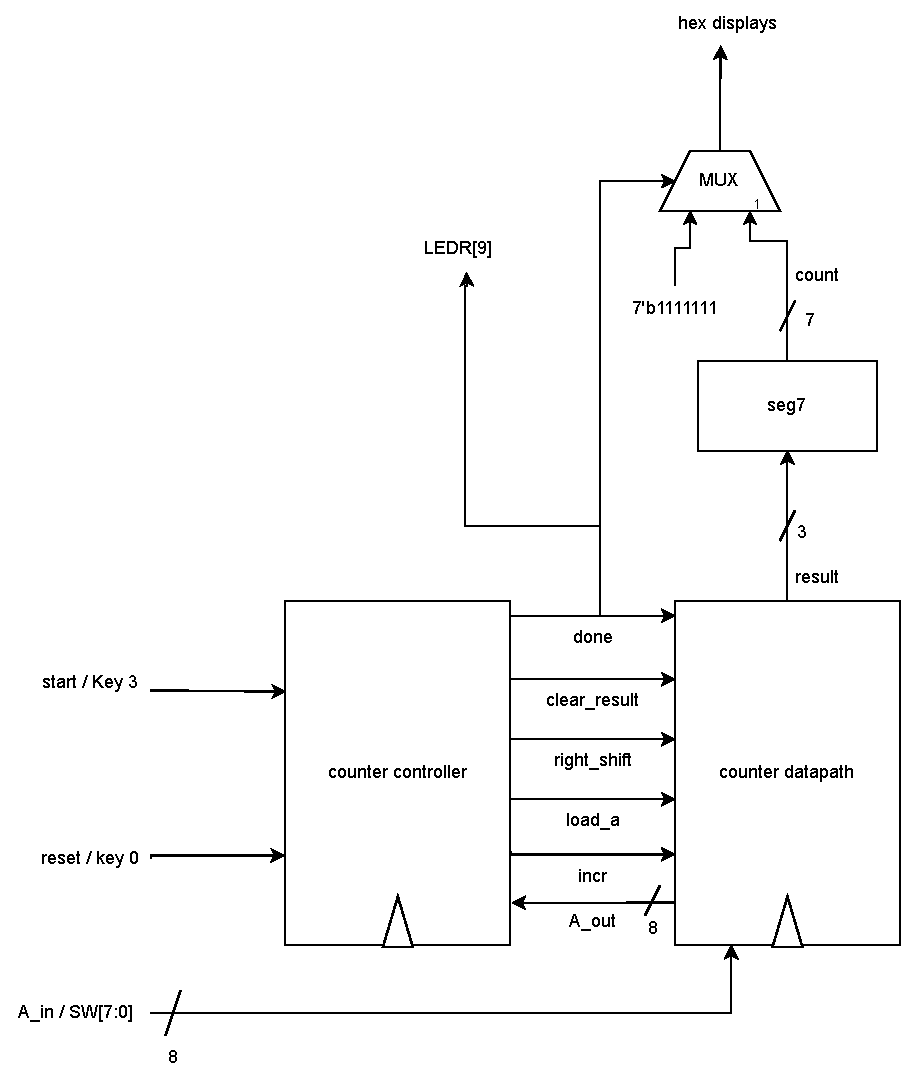
\includegraphics[scale=0.7]{Images/task 1 block diagram.pdf}
                \caption{Bit-counter block diagram}
            \end{figure}
            
            The system starts in an idle state, this state resets the system and monitors the input of the switches for the input number. Once the start button is pushed, the system locks in the input number from the switches and begins to conditionally test the first bit in the number and then shift over to the next bit until there are no more ones in the system, or A is equal to zero. The first step in the state is to check if A is equal to zero to then possibly move onto the next state. The system is then in the done state, this is signaled by the number of ones in the number being output on the HEX display and an LED turning on. The system can be reset again by toggling the start button or reset button.
        

        \subsection{Task \#2}
            The second and final task of this lab was to make a system that is able to search through an array of numbers using binary-search. Similar to task 1, an 8 bit number is input to the system on SW[7:0], KEY[3] for start, and KEY[0] for reset. The number given is searched for in a 32 element array that is implemented using a 32 address by 8 bit ROM file generated using the IP Catalog, the contents are initialized using a .mif file of random values. The system uses both HEX0 and HEX1 to display the element the number is in as well as LEDR[9] and LEDR[0] to display if the state is done and the number is found respectively.

            \begin{figure}[H]
                \centering
                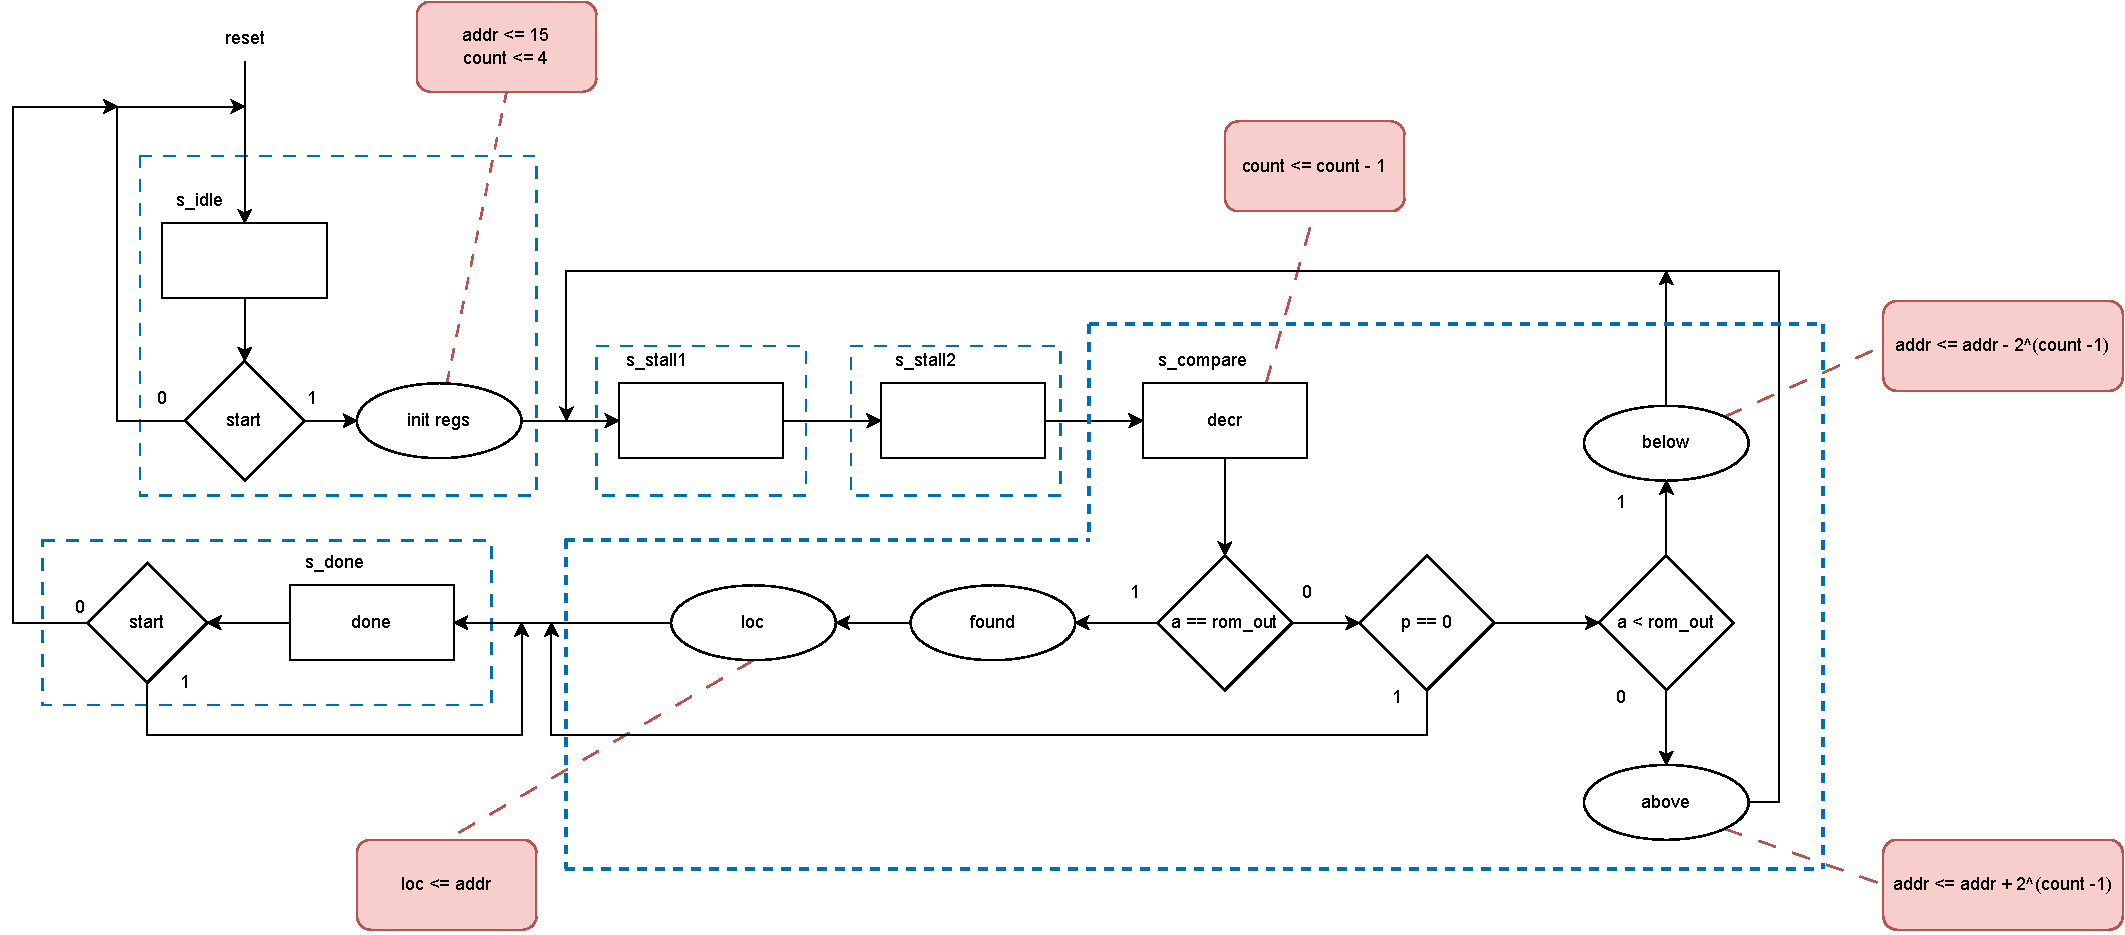
\includegraphics[scale = 0.45]{Images/task 2 asmd diagram.pdf}
                \caption{Binary search ASMD chart}
            \end{figure}

            \begin{figure}[H]
                \centering
                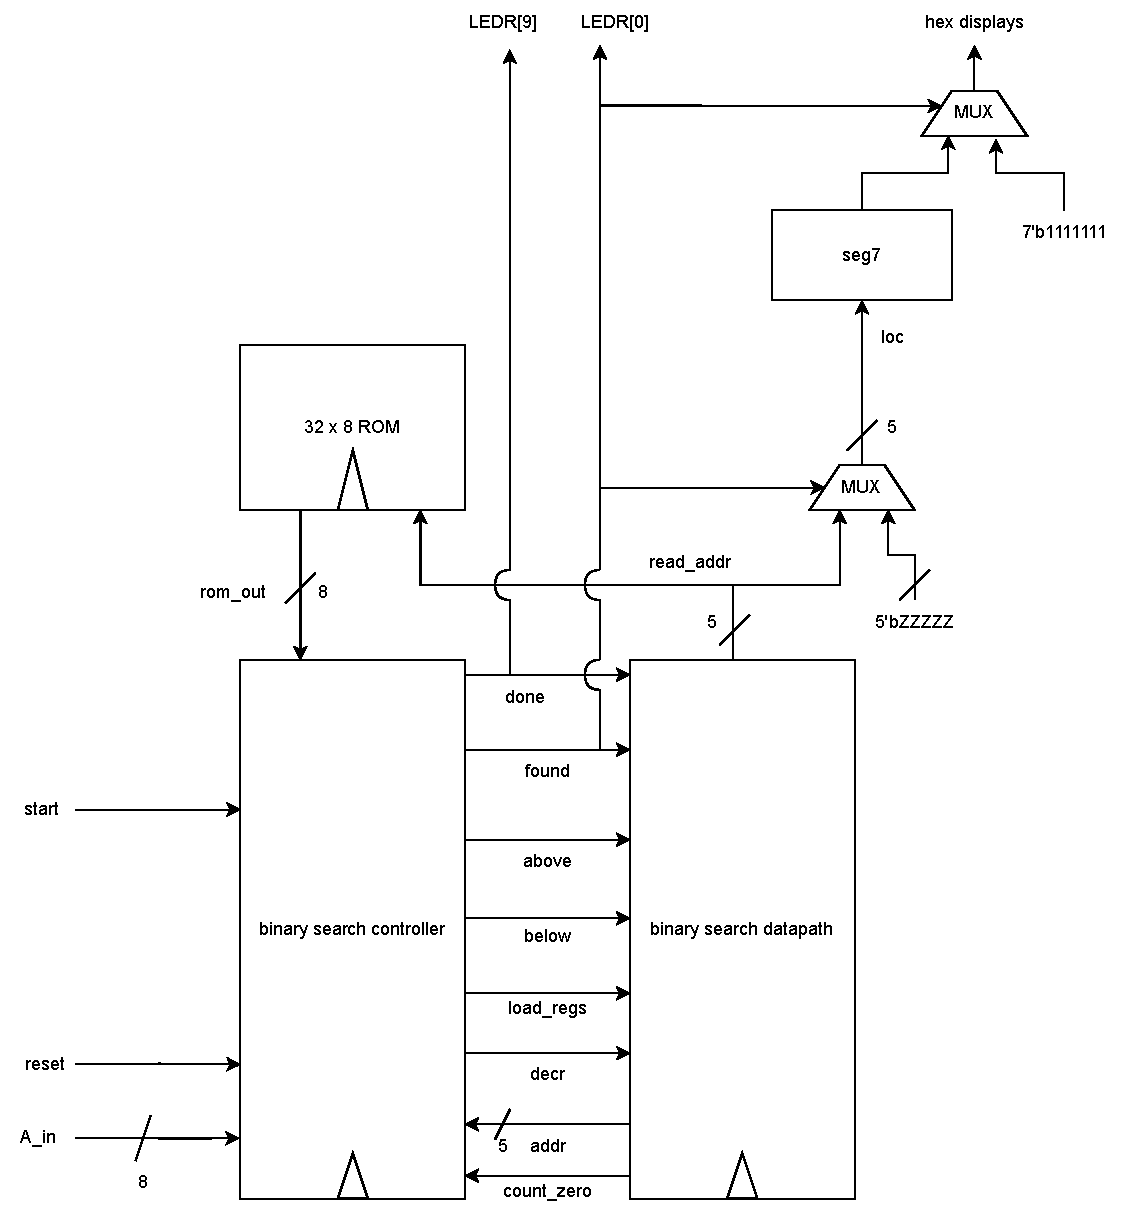
\includegraphics[scale=0.5]{Images/task 2 block diagram.pdf}
                \caption{Binary search block diagram}
            \end{figure}
            
            The system starts in the idle state which resets the data in the datapath back to their original values. Once the start signal is received from the DE1\_SoC board, the system moves to the internal states of the system that are used for searching. First there is a stall stage while an address is passed to the ROM's clocked register inputs. Then there is another stall stage while the output value from ROM is updated in the controller of the system. Finally, there is the compare stage which decides if we found our number and can move onto the done state, or if the bound has to be increased/decreased depending on the situation. In that case, the state of the system continues searching. The system can also determine if the number is not in the array depending on the count of searches it has unsuccessfully attempted, which is 5. If the number is found or not, the system moves into the done state which turns on LEDR[0] to display the system is done and possibly turns on LEDR[9] if the number is found. When the number is found, the HEX0 and HEX1 will display the address it was found in.

        \subsection{Overall System}
            The last step of the lab was to connect both the systems to the DE1\_SoC board and choose which one was running using SW[9]. Therefore the block diagram of the overall system would be similar to the following design:
            
            \begin{figure}[H]
                \centering
                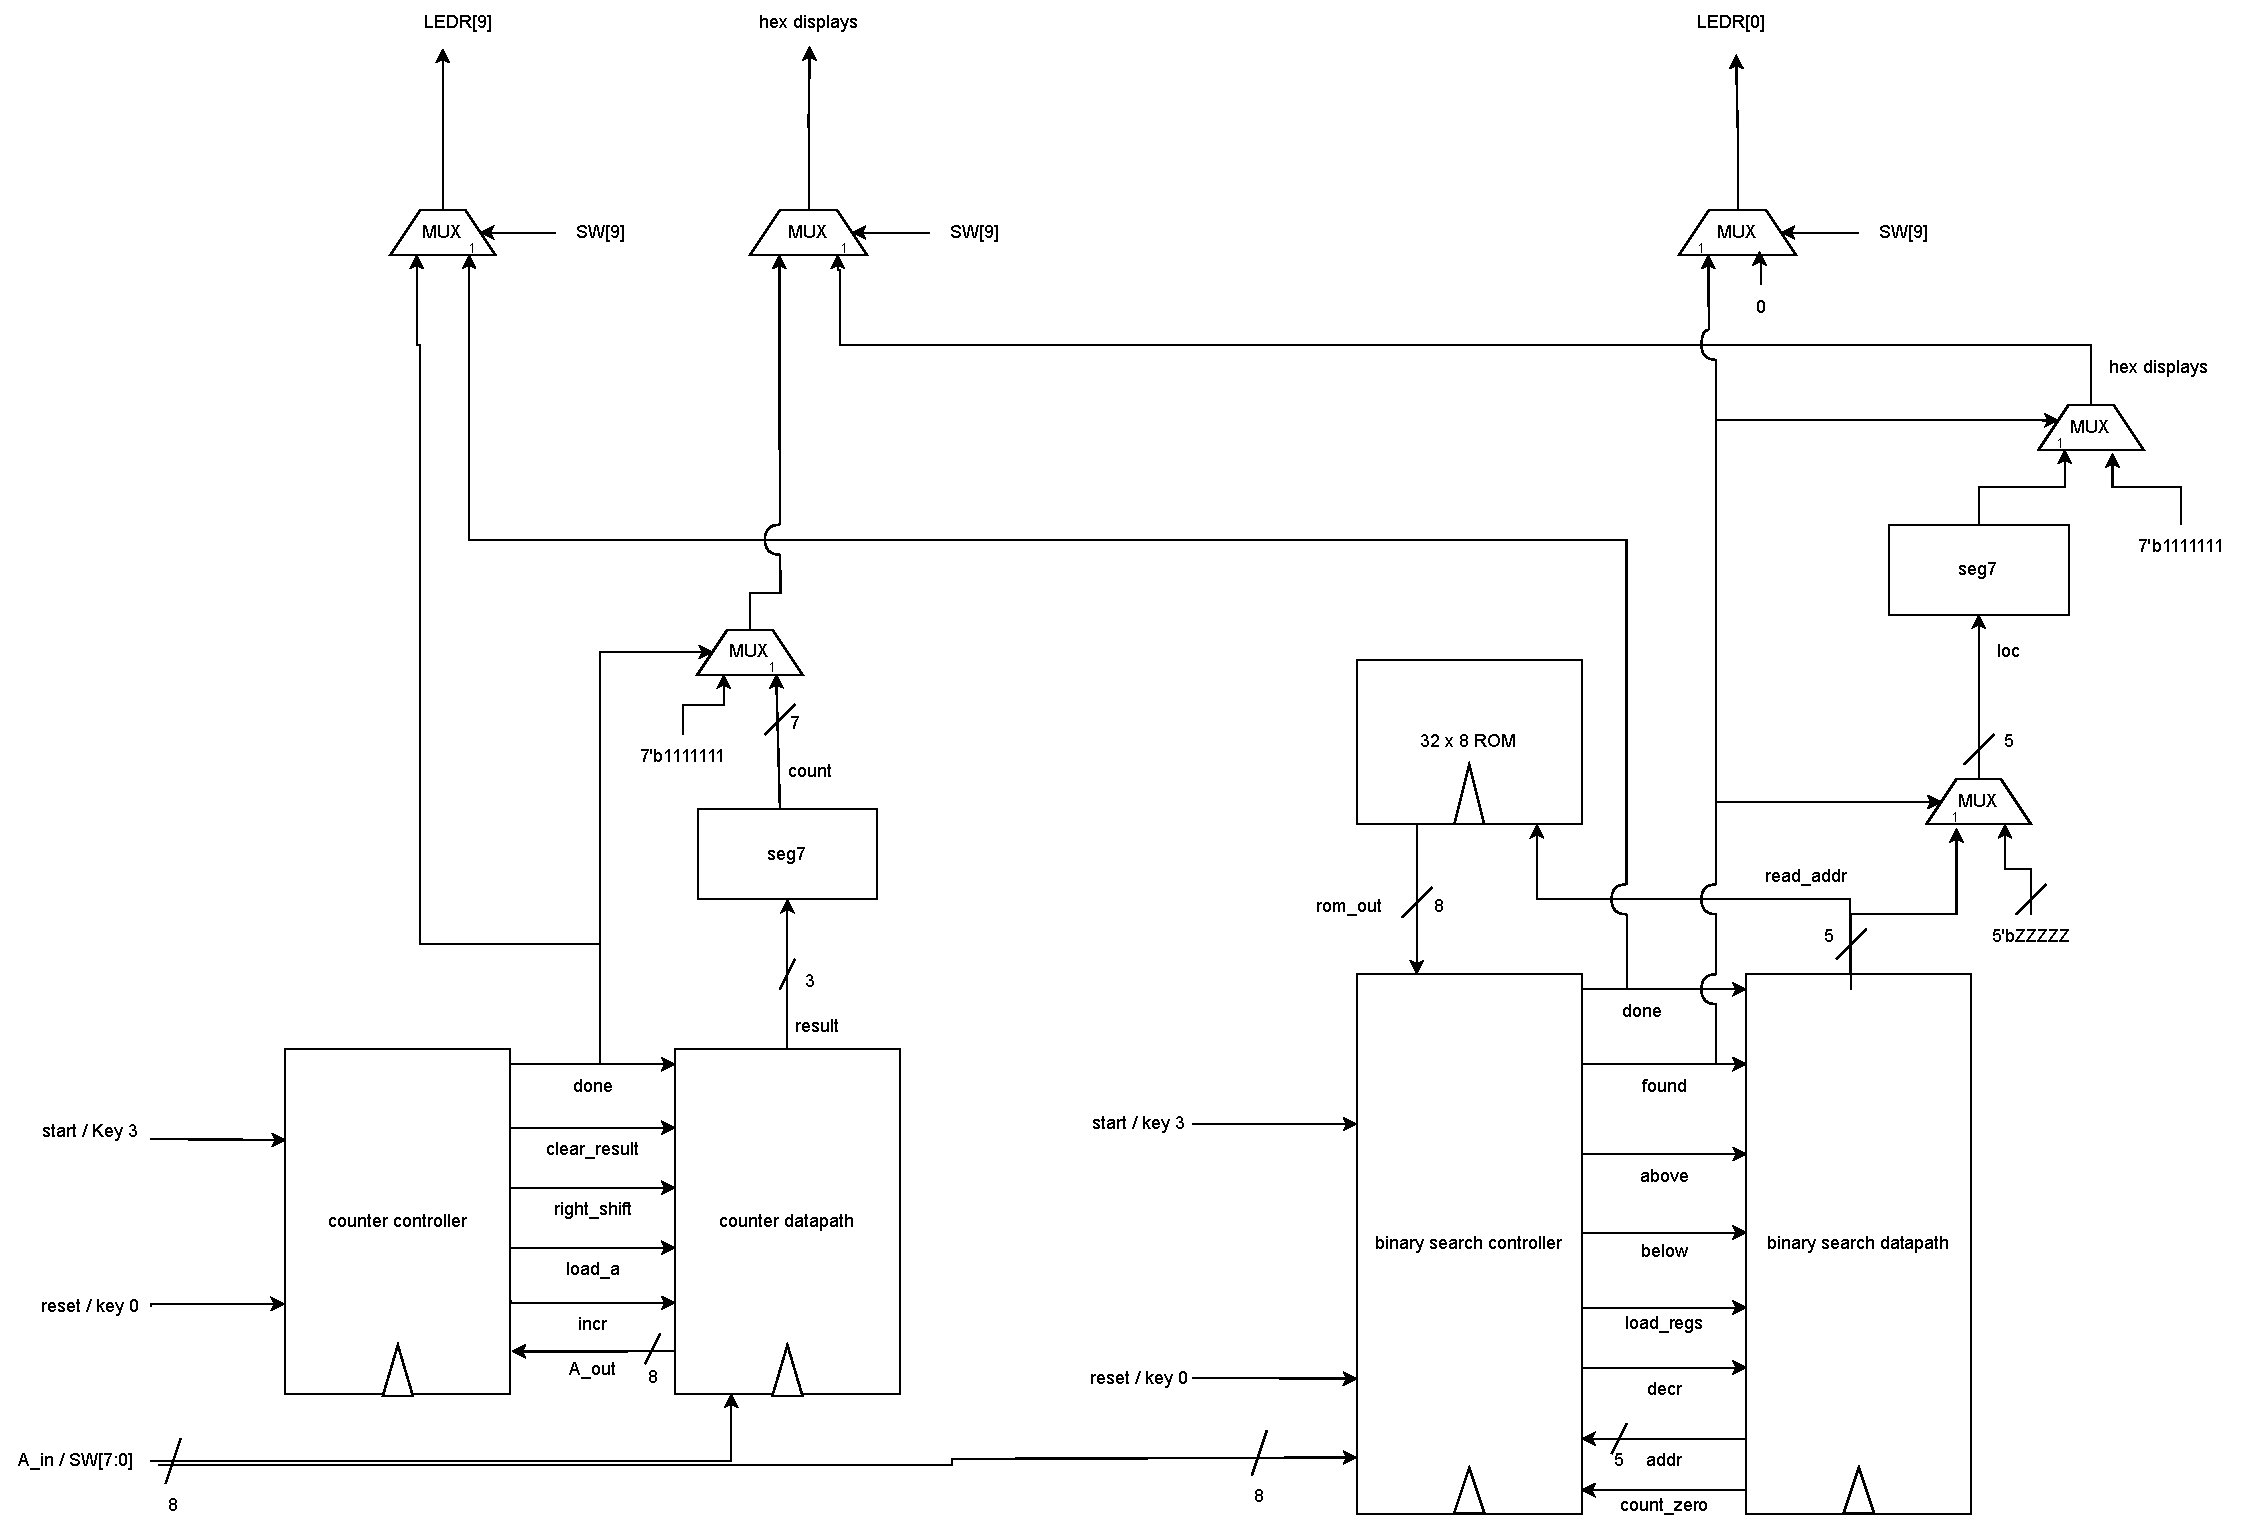
\includegraphics[scale=0.4]{Images/task 2 top level block diagram.pdf}
                \caption{Task 2 top level block diagram}
            \end{figure}

            This block diagram is pretty much just a combination of the individual block diagrams of the subparts. The outputs to displays and LEDs have MUXes so that they correctly show the information about the task that is currently running (based on SW[9]).
    \newpage
    \section{Results}
        The importance of this lab was becoming more familiar with implementing algorithms using hardware, which is a simplified process using a control and datapath to model the behavior. The systems that we implemented and tested are a bit-counting algorithm and a binary search algorithm. 

        \subsection{Bit-Counter Testbench}
            
            \begin{figure}[H]
                \centering
                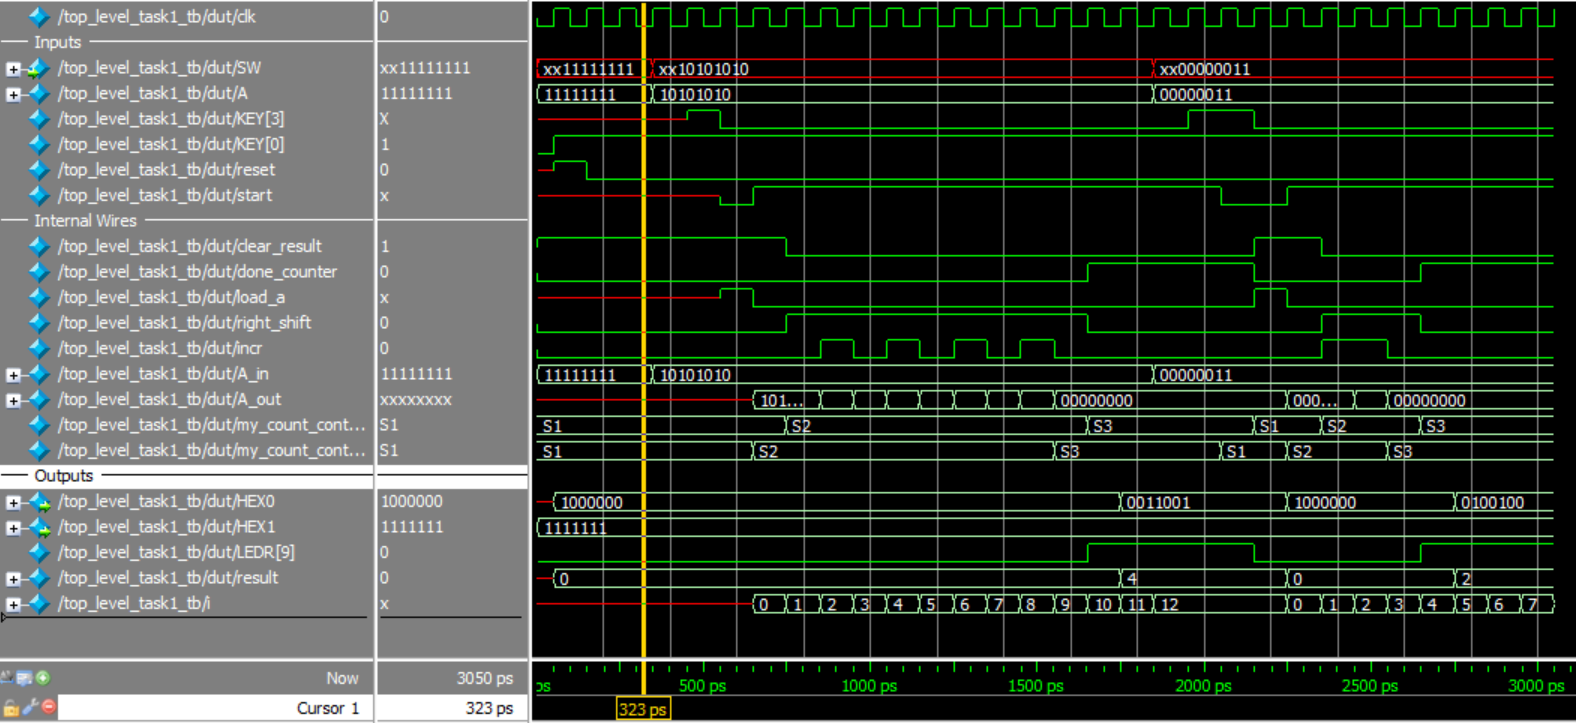
\includegraphics[scale=0.5]{Images/task 1 testbench.png}
                \caption{Task 1 Testbench}
            \end{figure}
            
            This testbench demonstrates the bit-counting algorithm. First, the system is reset, setting the system to the S1 state, or idle, where the clear result and load registers signals turn on for the datapath. The switches are then set and A updates on the next clock cycle, the switches are then changed again to show the load\_registers signal working in the idle state. The A in this case is 8'b10101010. The system receives the start signal and S2 state is turned on, or the shift and count stage. The first bit is checked, with the result increasing only if it is one, and then shifting the number logically to the right until A is equal to 0. Then the system moves on to the done state and results updates to 4, the LEDR[9] turns on, and HEX0 changes to represent the result. Then, start is turned off and the system goes back to S1 or idle, a new number is provided, and the system runs again. ``A'' in this case is 8'b00000011, so the program runs twice and dies, therefore the system runs as expected.
        \newpage

        \subsection{Binary Search Testbench}
            For the rest of the testbenches, the following mif file was used to initialize the ROM. 

            \begin{figure}[h]
                \centering
                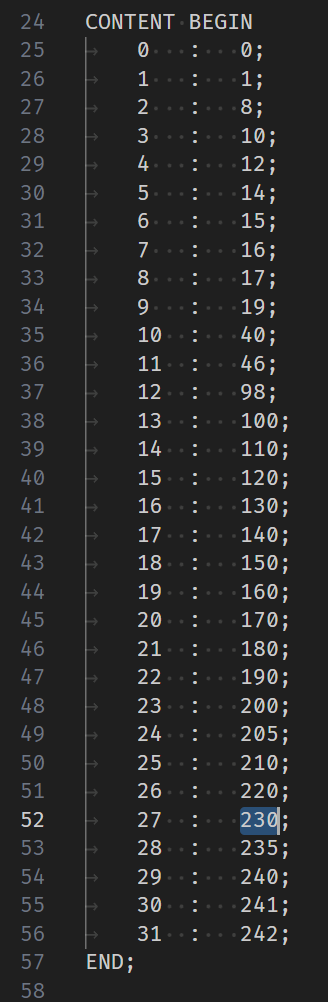
\includegraphics[scale=0.4]{Images/rom data.png}
                \caption{ROM mif file}
            \end{figure}

            Below is the testbench for the binary search part of task \# 2.
            \begin{figure}[H]
                \centering
                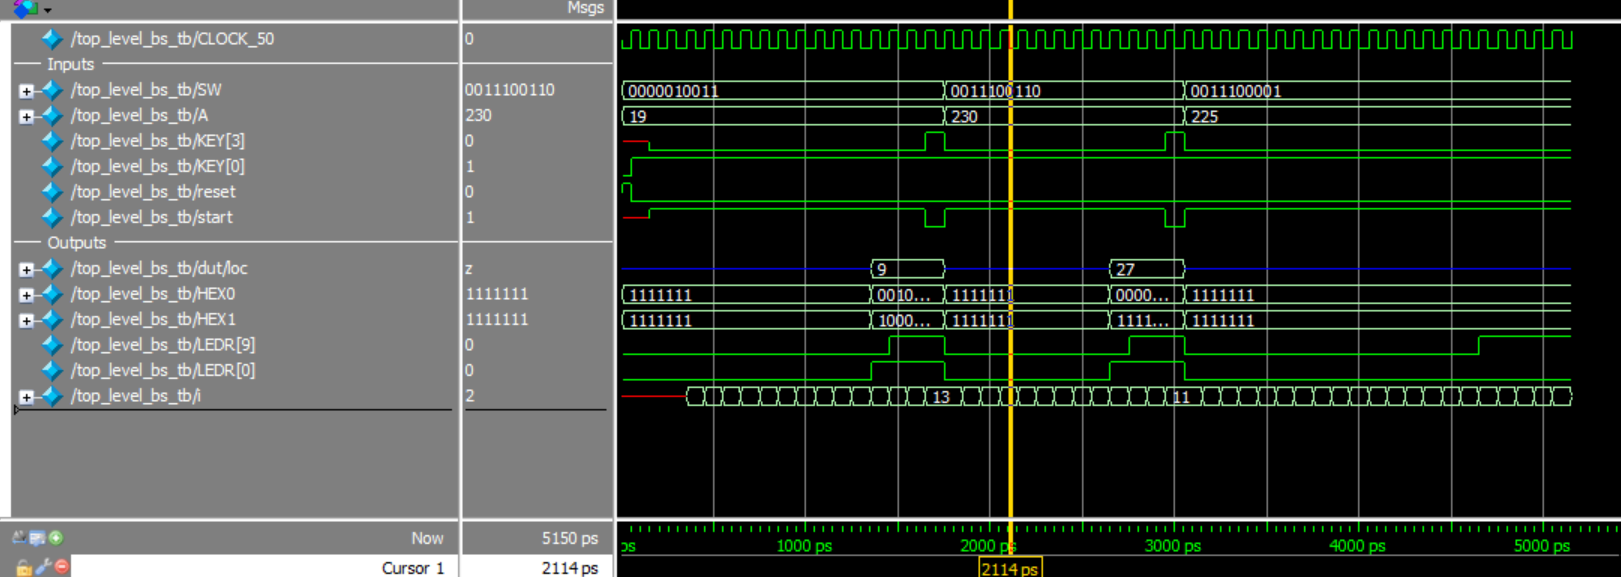
\includegraphics[scale=0.52]{Images/binary search testbench.png}
                \caption{Task 2 binary search testbench}
            \end{figure}
            This testbench demonstrates that the binary search is correct. It shows that the binary search correctly finds the value \texttt{19} at address \texttt{9}. It also shows that the HEX displays update to the address once the value has found. It demonstrates searching for a different value, \texttt{230}. It also demonstrates searching for a value which is not in the ROM. In that case, the module correctly sets the LEDs to show that the algorithm has finished running but didn't find the value. It also sets the displays to show nothing because no address held the value. This demonstrates the expected behavior. 

        \newpage
        \subsection{Task \#2 Top-level Testbench}
            This test bench demonstrates the top-level module in task \#2 works correctly.

            \begin{figure}[H]
                \centering
                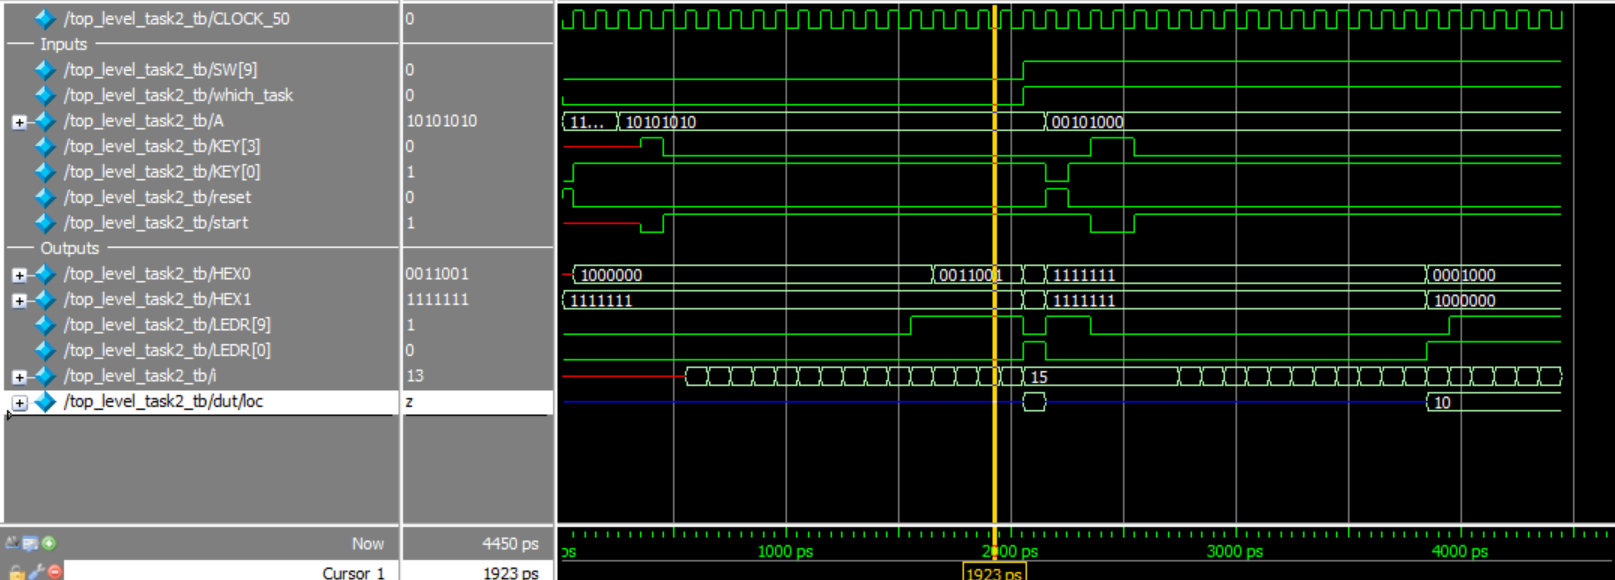
\includegraphics[scale=0.52]{Images/binary search top level testbench.png}
                \caption{Task 2 top-level testbench}
            \end{figure}
            This testbench shows that the circuit correctly counts the number of bits in SW[7:0], which is 4. It then properly updates the HEX display to display 4 and turns on LEDR[9] to show the algorithm is finished running. When SW[9] is flipped, the circuit then changes to binary searching. SW[7:0] is then changed to 40, meaning the circuit should search for the value 40. After it finished searching, the LEDs are updated to show the algorithm finished running and the value was found. The HEX displays also change to display the address the value was found at. This shows the expected behavior. 
        \newpage
        \subsection{Flow Summary}
            \begin{description}
                \item \textbf{Task 1} \\
                    Analysis \& Synthesis Status : Successful - Sun Nov  5 00:01:34 2023 \\
                    Quartus Prime Version : 17.1.0 Build 590 10/25/2017 SJ Lite Edition \\
                    Revision Name : top\_level\_task1 \\
                    Top-level Entity Name : top\_level\_task1 \\
                    Family : Cyclone V \\
                    Logic utilization (in ALMs) : N/A \\
                    Total registers : 16 \\
                    Total pins : 39 \\
                    Total virtual pins : 0 \\
                    Total block memory bits : 0 \\
                    Total DSP Blocks : 0 \\
                    Total HSSI RX PCSs : 0 \\
                    Total HSSI PMA RX Deserializers : 0 \\
                    Total HSSI TX PCSs : 0 \\
                    Total HSSI PMA TX Serializers : 0 \\
                    Total PLLs : 0 \\
                    Total DLLs : 0 \\

                    Fitter Status : Successful - Sat Nov  4 22:56:19 2023 \\
                    Quartus Prime Version : 17.1.0 Build 590 10/25/2017 SJ Lite Edition \\
                    Revision Name : top\_level\_task1 \\
                    Top-level Entity Name : top\_level\_task1 \\
                    Family : Cyclone V \\
                    Device : 5CSEMA5F31C6 \\
                    Timing Models : Final \\
                    Logic utilization (in ALMs) : 17 / 32,070 ( < 1 \% ) \\
                    Total registers : 18 \\
                    Total pins : 39 / 457 ( 9 \% ) \\
                    Total virtual pins : 0 \\
                    Total block memory bits : 0 / 4,065,280 ( 0 \% ) \\
                    Total RAM Blocks : 0 / 397 ( 0 \% ) \\
                    Total DSP Blocks : 0 / 87 ( 0 \% ) \\
                    Total HSSI RX PCSs : 0 \\
                    Total HSSI PMA RX Deserializers : 0 \\
                    Total HSSI TX PCSs : 0 \\
                    Total HSSI PMA TX Serializers : 0 \\
                    Total PLLs : 0 / 6 ( 0 \% ) \\
                    Total DLLs : 0 / 4 ( 0 \% )
                
                \newpage
                \item \textbf{Task 2} \\
                    Analysis \& Synthesis Status : Successful - Sun Nov  5 06:59:08 2023 \\
                    Quartus Prime Version : 17.1.0 Build 590 10/25/2017 SJ Lite Edition \\
                    Revision Name : top\_level\_task2 \\
                    Top-level Entity Name : top\_level\_task2 \\
                    Family : Cyclone V \\
                    Logic utilization (in ALMs) : N/A \\
                    Total registers : 27 \\
                    Total pins : 39 \\
                    Total virtual pins : 0 \\
                    Total block memory bits : 256 \\
                    Total DSP Blocks : 0 \\
                    Total HSSI RX PCSs : 0 \\
                    Total HSSI PMA RX Deserializers : 0 \\
                    Total HSSI TX PCSs : 0 \\
                    Total HSSI PMA TX Serializers : 0 \\
                    Total PLLs : 0 \\
                    Total DLLs : 0 \\

                    Fitter Status : Successful - Sun Nov  5 06:59:39 2023 \\
                    Quartus Prime Version : 17.1.0 Build 590 10/25/2017 SJ  Lite Edition \\
                    Revision Name : top\_level\_task2 \\
                    Top-level Entity Name : top\_level\_task2 \\
                    Family : Cyclone V \\
                    Device : 5CSEMA5F31C6 \\
                    Timing Models : Final \\
                    Logic utilization (in ALMs) : 49 / 32,070 ( < 1 \% ) \\
                    Total registers : 27 \\
                    Total pins : 39 / 457 ( 9 \% ) \\
                    Total virtual pins : 0 \\
                    Total block memory bits : 256 / 4,065,280 ( < 1 \% ) \\
                    Total RAM Blocks : 1 / 397 ( < 1 \% ) \\
                    Total DSP Blocks : 0 / 87 ( 0 \% ) \\
                    Total HSSI RX PCSs : 0 \\
                    Total HSSI PMA RX Deserializers : 0 \\
                    Total HSSI TX PCSs : 0 \\
                    Total HSSI PMA TX Serializers : 0 \\
                    Total PLLs : 0 / 6 ( 0 \% ) \\
                    Total DLLs : 0 / 4 ( 0 \% ) \\
            \end{description}
            
    \newpage
    \section{Experience Report}
        This lab was harder, it took a while at first to review implementations of control and datapath modules from lecture. However, once that was figured out the ASMD chart was simple to follow for the first task and generating one for task two was not too challenging either. Implementing task 2 was hard though. Figuring out timing issues with the ROM was difficult and took a significant amount of time to debug. Another challenge we encountered was trying to run the two tasks on the same board, but now that we found a method to do so the next labs we will be able to use our experience.
    

        This lab took approximately 16 hours, broken down as follows:
        \begin{description}
            \item[Reading:] 45 minutes
            \item[Design:] 15 minutes
            \item[Coding:] 7 hours
            \item[Debugging:] 5 hours
            \item[Write up:] 3 hours
        \end{description}   
        
\end{document}
